En este capítulo se presentan los resultados obtenidos al procesar las señales y se realiza un breve análisis. Al registrar sesiones, o bien se creaba una sesión de entrenamiento y una de predicción, en la que se evaluaba el desempeño, o bien se creaba una única sesión y luego se dividía en dos partes. Debido a que el posicionamiento del sensor es importante y varía cuando se coloca y se retira,  y a que el estado del cuerpo cambia de un instante al otro, las bioseñales sufren variaciones. Por este motivo, las sesiones de entrenamiento y predicción se registraban una a continuación de la otra. De esta manera, se buscaba que la señal sea lo más consistente posible.

\section{EEG}

Como se mencionó en la sección \ref{sec:eeg-signal-processing} del capítulo anterior, primero se comenzó utilizando los valores de potencia \emph{Alfa} que brindaba el sensor ($\alpha_{10 \, Hz}$). Como no se lograba el nivel de precisión deseado, se decidió realizar una implementación propia ($\alpha_{256 \, Hz}$) y confeccionar el vector de características con cuatro elementos. En la tabla \ref{tab:eeg-results} se pueden observar los resultados de aplicar ambos métodos a distintas sesiones de entrenamiento de distintos sujetos.

\begin{table}[H]
\centering
\begin{tabular}{ |c|c|c|c| } 
 \hline
 Sujeto & Sesión & $\alpha_{10 \, Hz}$ &  $\alpha_{256 \, Hz}$ \\ 
 \hline
 1 & 1 & $0.5659229$ & $0.6910995$ \\
 \hline
 1 & 2 & $0.6265357$ & $0.672956$ \\
  \hline
 2 & 1 & $0.6808835$ & $0.8532819$ \\
  \hline
 2 & 2 & $0.6527051$ & $0.8533725$ \\

 \hline
\end{tabular}
\caption{Resultados de utilizar distintas formas de calcular potencia de \emph{Alfa} en distintos sujetos.}
\label{tab:eeg-results}
\end{table}

La primer observación que se puede realizar es que utilizar $\alpha_{256 \, Hz}$ es más preciso que utilizar $\alpha_{10 \, Hz}$. Como se mencionó anteriormente, esto se debe a que en el primer caso se toman $256$ muestras para calcular la potencia de \emph{Alfa} mientras que en el segundo se utilizan únicamente $25$. A su vez, en el primer caso se utilizan los valores obtenidos por cada electrodo por separado mientras que en el segundo caso se promedian y se arma el vector de características con dos valores consecutivos. Utilizar las mediciones de los distintos electrodos en un período de tiempo describe mejor el estado que utilizar valores de dos períodos consecutivos.

En las figuras \ref{fig:subject-2-10} y \ref{fig:subject-2-256} se observan gráficos de dispersión utilizando los valores de potencia de \emph{Alfa}. En ambos se observa una clara separación de estados. El estado de ojos cerrados contiene valores mayores que el estado de ojos abiertos. La figura \ref{fig:subject-2-10}  cuenta con una cantidad mayor de valores atípicos, particularmente, una cantidad mayor de valores de \emph{Alfa} elevados en el estado de ojos abiertos. A su vez, en la figura \ref{fig:subject-2-256} los valores para ojos abiertos se encuentran mayormente concentrados por debajo de los valores para ojos cerrados. Por estos motivos, la precisión es mucho mayor al utilizar el vector de cuatro dimensiones.

 \begin{figure}[H]
	\centering
    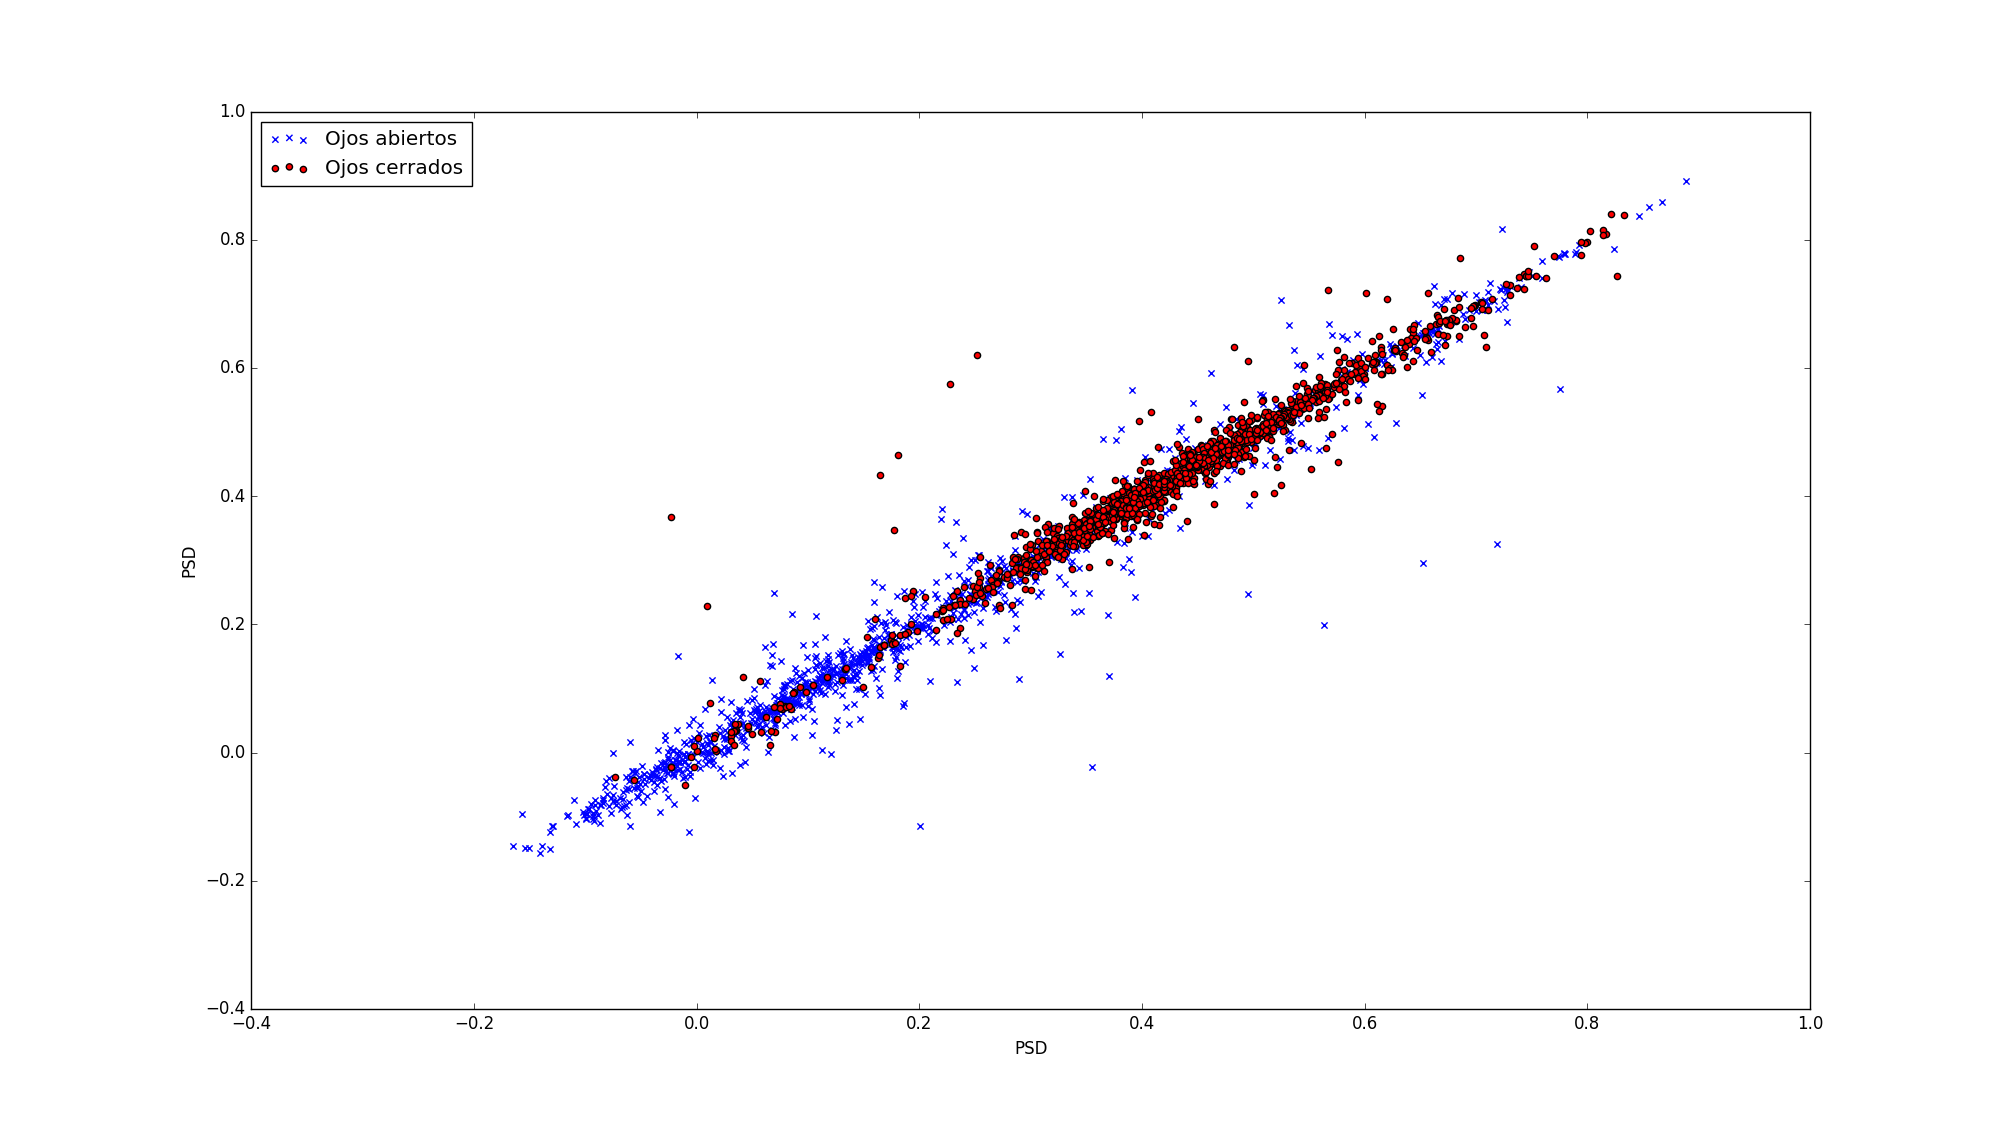
\includegraphics[width=0.8\textwidth]{subject-2-10.png}
    \caption{Gráfico de dispersión del vector de características de dos características de la sesión  2 del sujeto 2.}
	\label{fig:subject-2-10}
\end{figure}

 \begin{figure}[H]
	\centering
    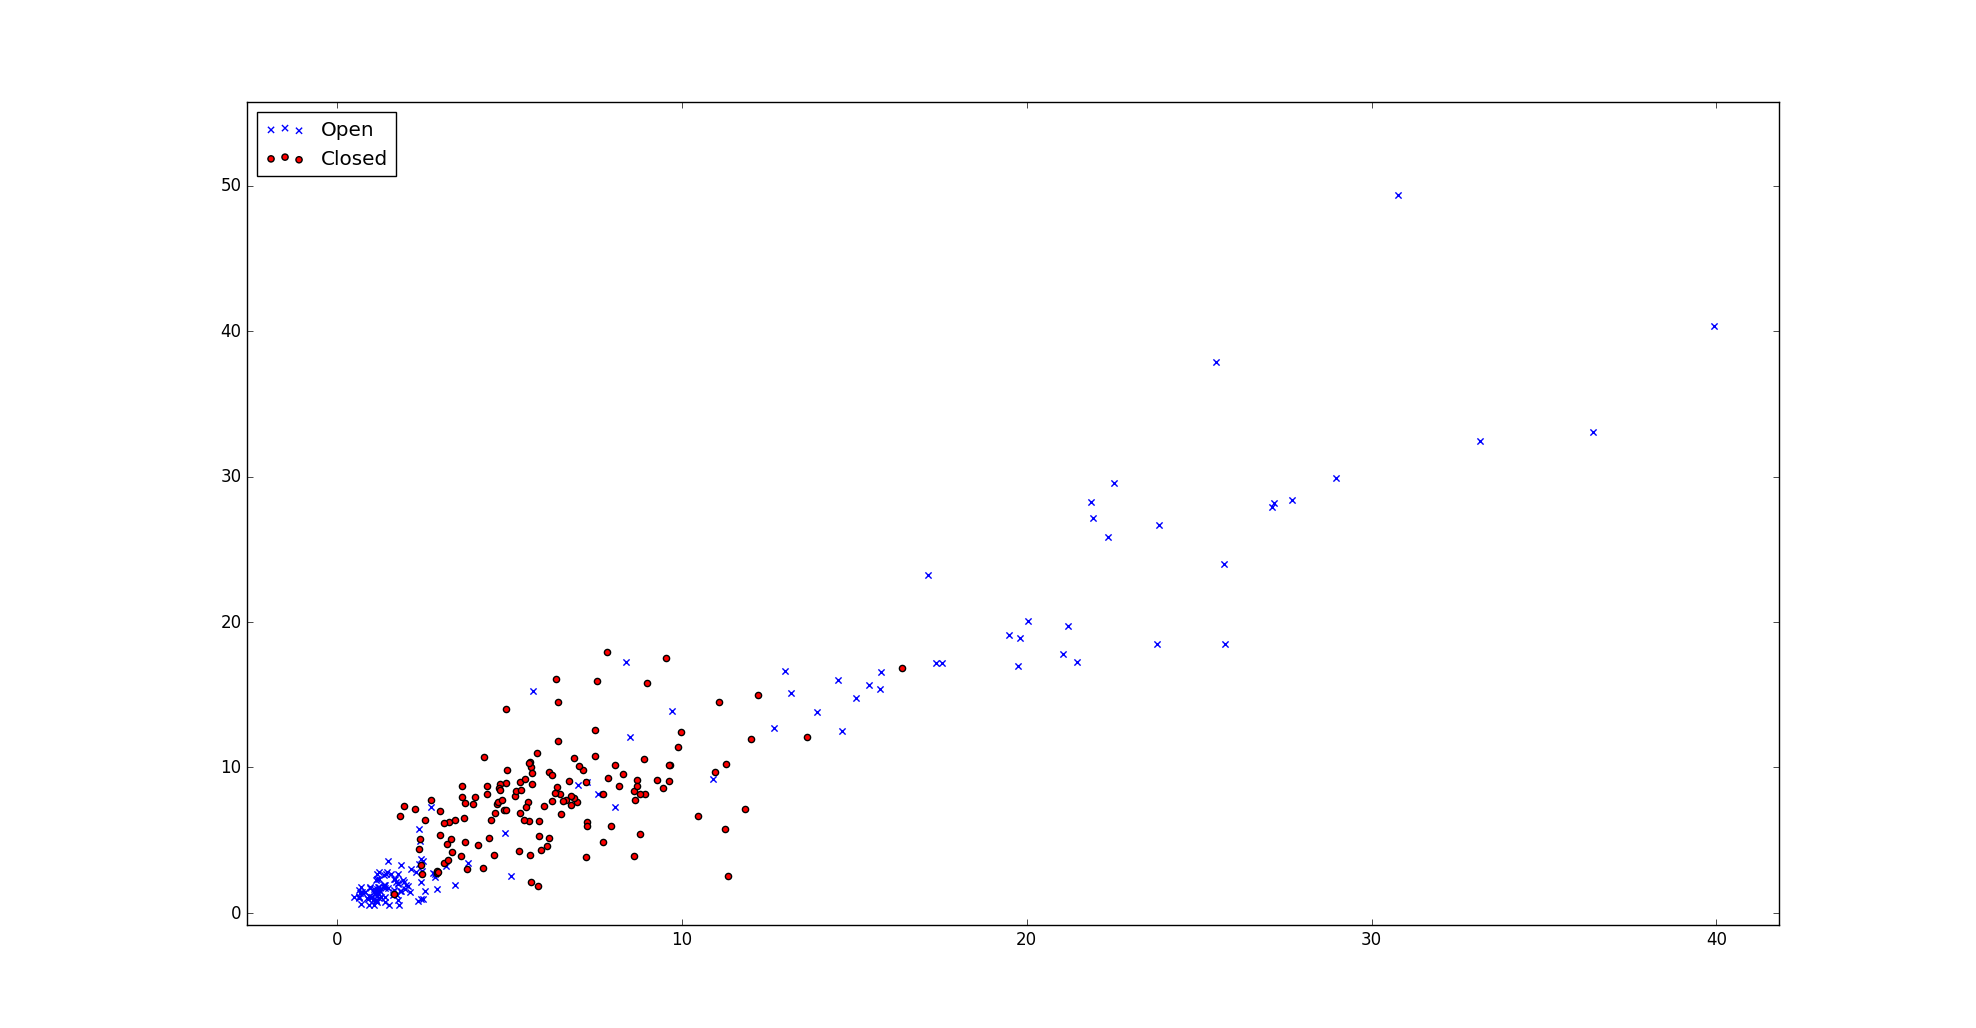
\includegraphics[width=0.8\textwidth]{subject-2-256.png}
    \caption{Gráfico de dispersión del vector de características de cuatro características de la sesión  2 del sujeto 2. Para transformar de cuatro dimensiones a dos, se promediaron los dos primeros valores y los dos valores finales.}
	\label{fig:subject-2-256}
\end{figure}

Cabe destacar que al contar con un vector de cuatro características, para graficar se necesitarían cuatro dimensiones. Para abordar este problema se decidió transformar el vector en un vector de dos componentes donde la primer componente es el promedio de los dos primeros valores y la segunda, el promedio de los dos últimos valores.

Otro aspecto a analizar es el hecho de que la precisión varía mucho de sujeto a sujeto. Esto puede deberse a diversos motivos. Uno de ellos es que la persona al saber que está siendo analizada, se encuentra nerviosa por lo que puede afectar las ondas cerebrales. A su vez, si la persona se encuentra cansada, por ejemplo, los estímulos al campo visual tienden a ser menores, lo que genera que lo valores de \emph{Alfa} sean mayores.

Si bien las ondas cerebrales varían mucho de persona a persona y de acuerdo al instante del tiempo, se realizó la prueba de utilizar como sesión de entrenamiento una sesión del sujeto 2 (sesión 2) y como sesión de predicción una sesión del sujeto 1 (sesión 1). Los resultados fueron sorprendentes ya que se obtuvo una precisión de $0.6963351$. Esta fue superior a la precisión obtenida con la sesión de entrenamiento del propio sujeto. De esta forma, se observa que el sistema de clasificación ofrece un determinado nivel de robustez.

\section{EMG}

Como se mencionó en la sección \ref{sec:emg-signal-processing}, los valores leídos fueron procesados para obtener un vector de dos características cada $128$ muestras, y luego fueron alimentados a un clasificador. En la siguiente tabla se detalla: el sujeto utilizado, la precision alcanzada luego de entrenar al clasificador, y la duración total en segundos de las muestras tomadas.

\begin{table}[H]
\centering
\begin{tabular}{ |c|c|c|c| } 
 \hline
 Sujeto & Sesión & Precisión & Duración (Segundos) \\ 
 \hline
 1 & 1 & $0.994$ & $341$ \\
 \hline
 1 & 2 & $0.974$ & $603$ \\
 \hline
 1 & 3 & $0.976$ & $334$ \\
 \hline
 1 & 4 & $0.987$ & $299$ \\
  \hline
 2 & 1 & $0.892$ & $239$ \\
  \hline
 3 & 1 & $0.990$ & $393$ \\

 \hline
\end{tabular}
\caption{Resultados de entrenamientos utilizando lecturas de EMG para varios sujetos.}
\label{tab:emg-results}
\end{table}

Como muestran los valores de la tabla \ref{tab:emg-results}, los niveles de precisión alcanzados son muy elevados: en cinco de las seis sesiones realizadas, se logró un nivel de precisión de $97\%$, o mayor.  En la sesión del sujeto $2$, se logró un nivel más bajo, de $89\%$. Esto se debe, probablemente, a que ésta sesión tuvo una duración mas corta que las anteriores, por lo que el clasificador fue entrenado con un número menor de muestras. También es necesario remarcar que al medir señales de EMG, existen varias fuentes de ruido eléctrico, que pueden afectar los valores leídos y por lo tanto perjudicar la precision del entrenador. El efecto neto de éstas fuentes de ruido varía de sesión en sesión, ya que depende de factores como la cantidad de movimiento de los electrodos en relación a la piel, o la presencia de dispositivos que emitan radiación electromagnética\cite{emg-delsys}.

A continuación, se muestran los gráficos de dispersión de las dos sesiones más largas, que permiten visualizar las diferencias entre los vectores de características de ambos estados de tensión de músculo.

 \begin{figure}[H]
	\centering
    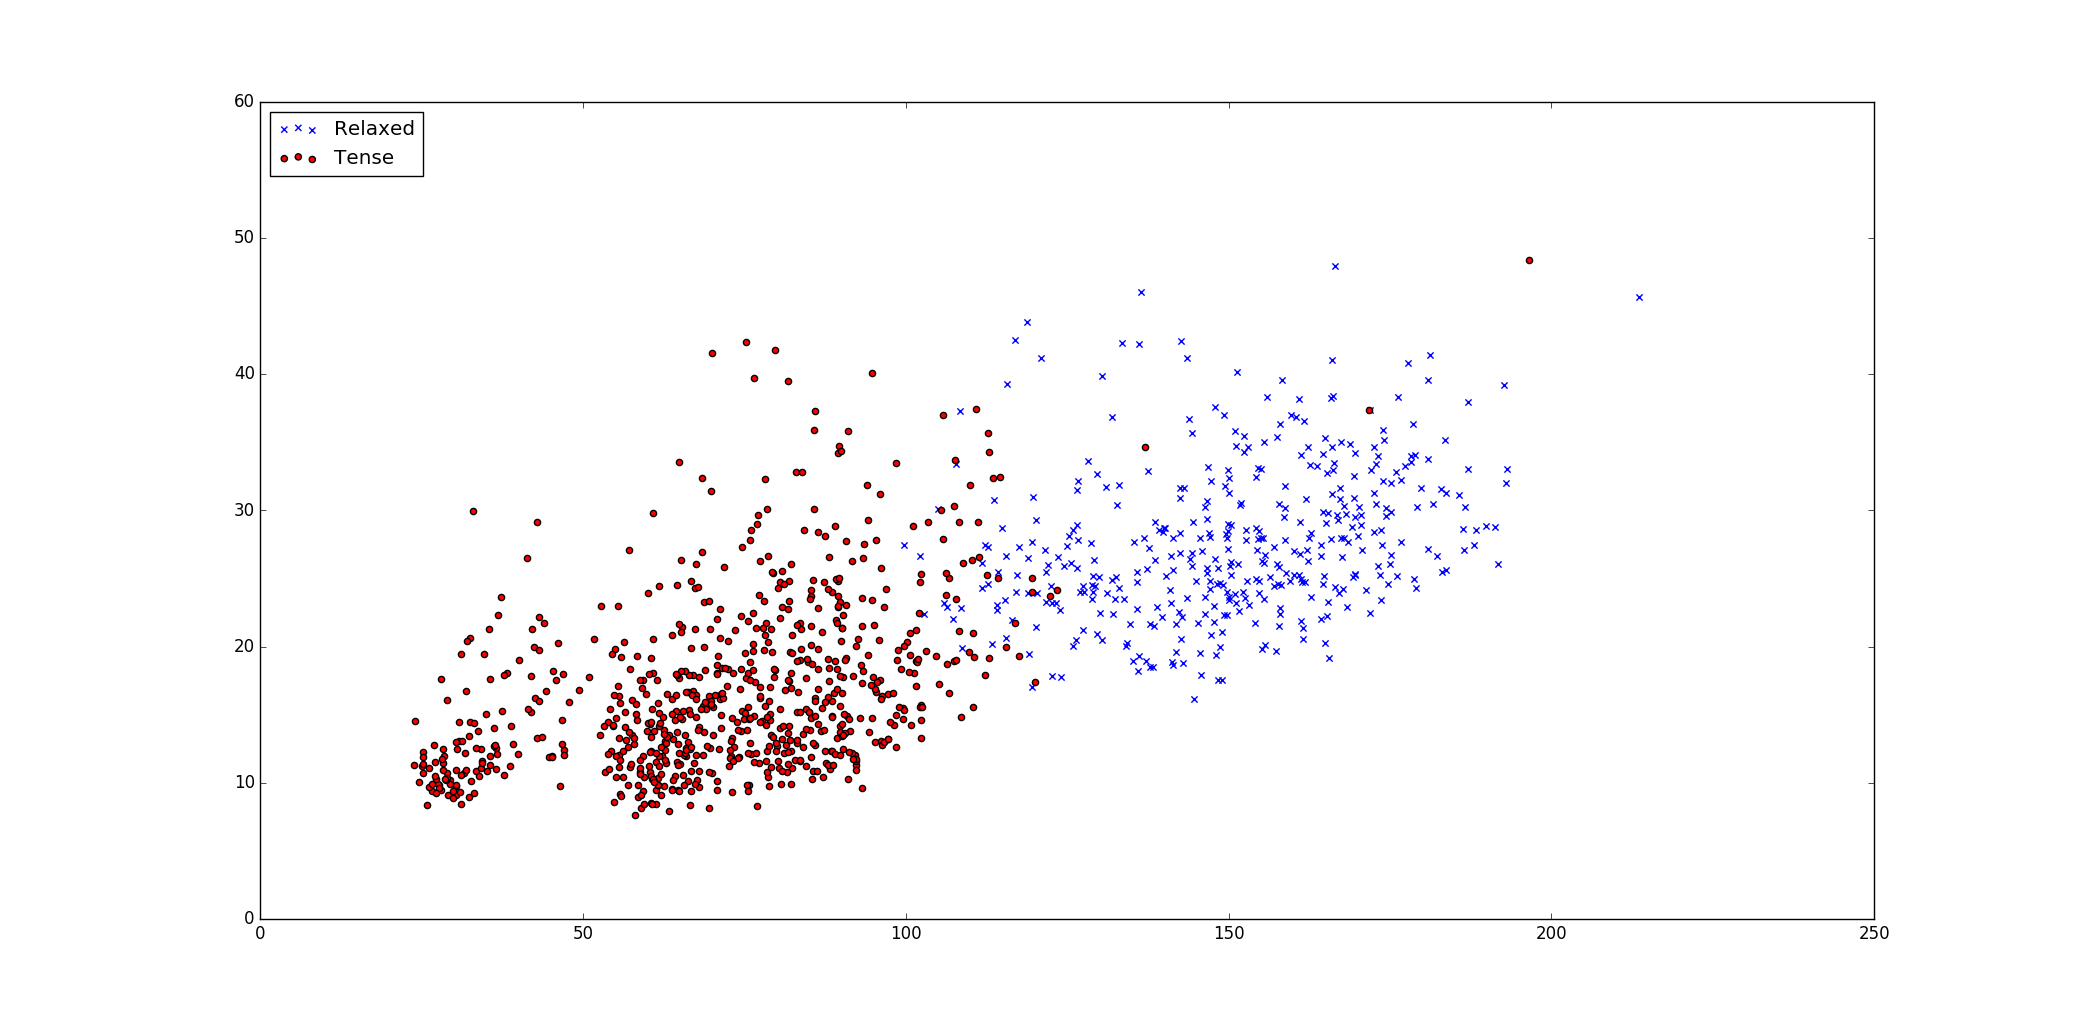
\includegraphics[width=1\textwidth]{fede-2.png}
    \caption{Gráfico de dispersión del vector de características EMG para la sesión $2$ del sujeto $1$.}
	\label{fig:emg-graph-s1s2}
\end{figure}

 \begin{figure}[H]
	\centering
    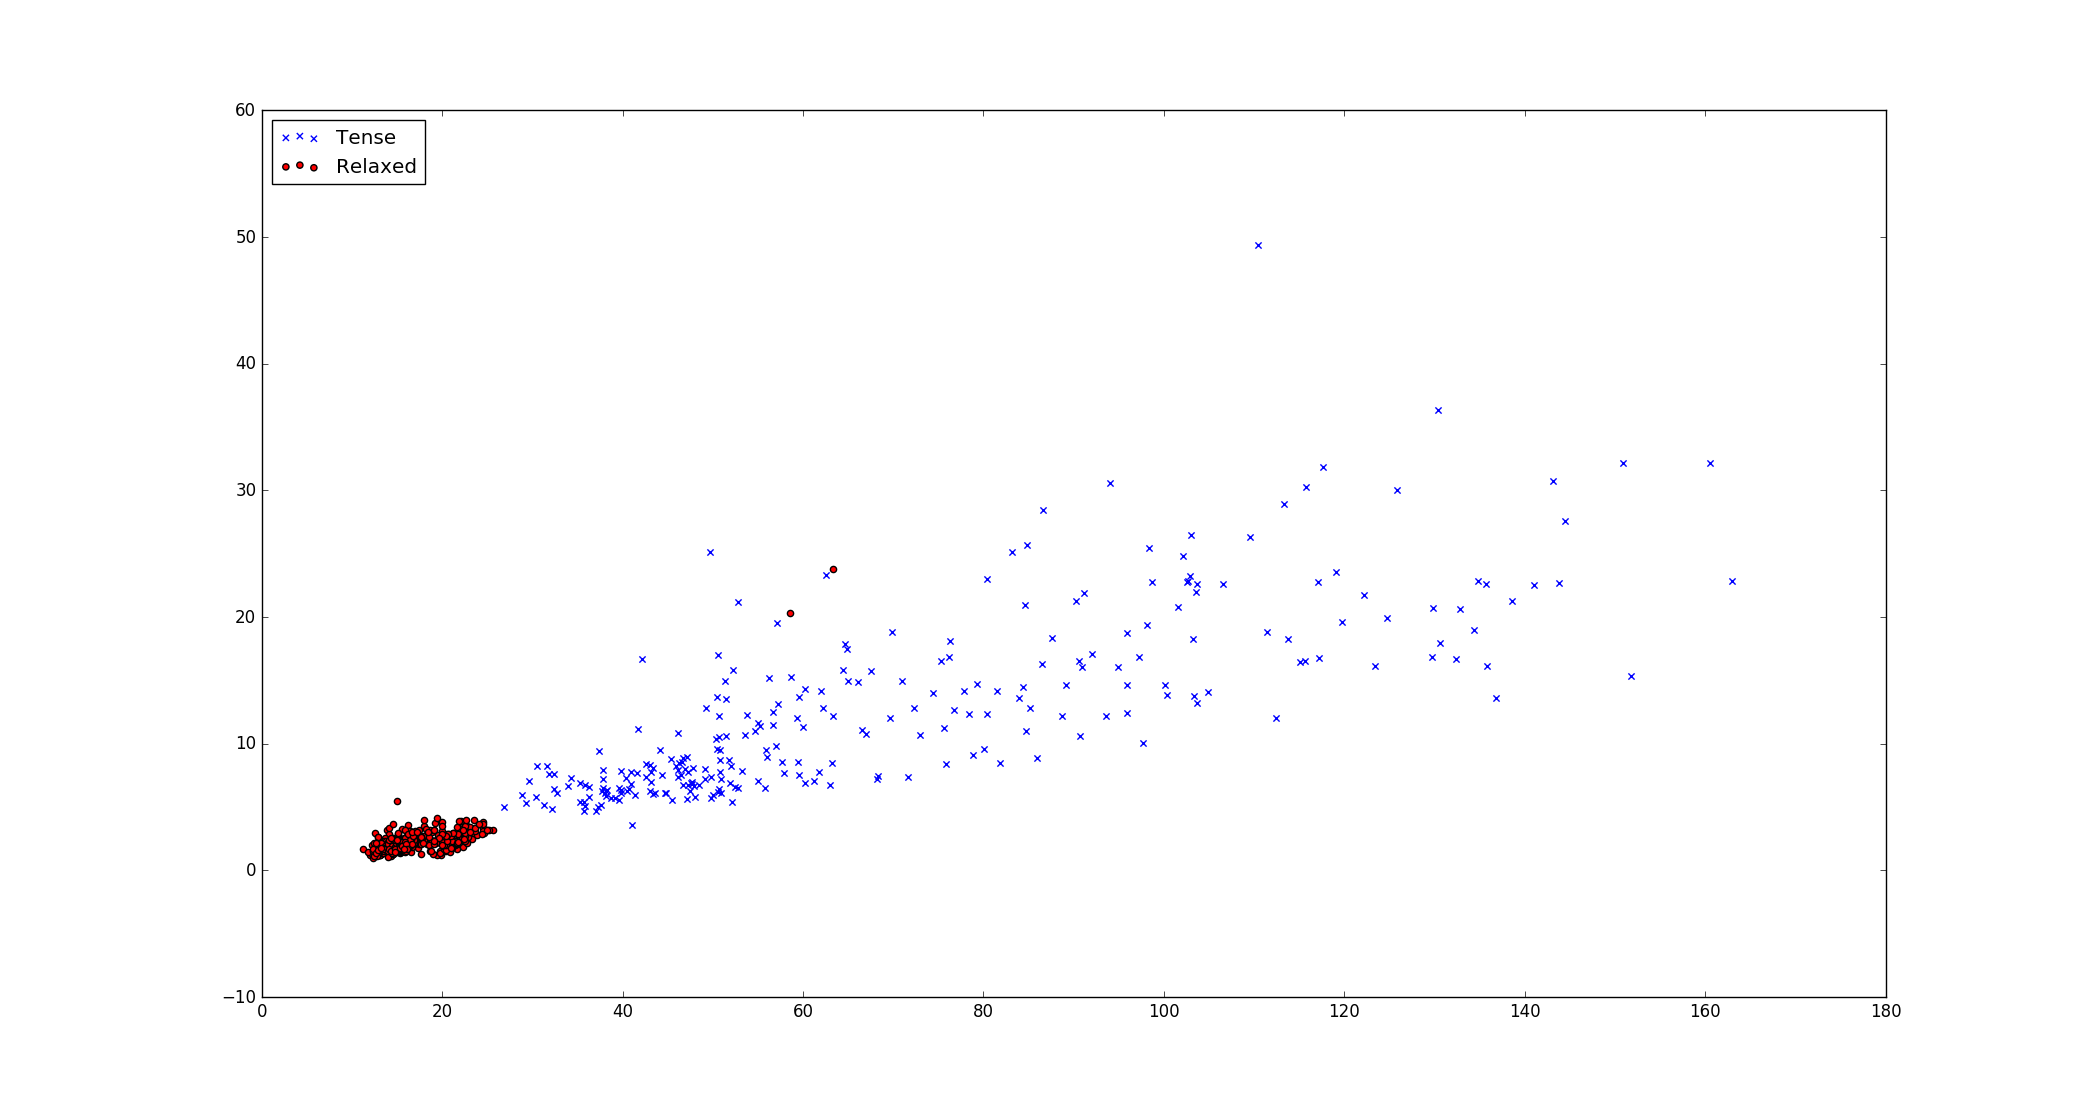
\includegraphics[width=1\textwidth]{javo-1.png}
    \caption{Gráfico de dispersión del vector de características EMG para la sesión $1$ del sujeto $3$.}
	\label{fig:emg-graph-s3s1}
\end{figure}

En la figura \ref{fig:emg-graph-s1s2}, se puede observar una clara separación entre las muestras tomadas con el musculo relajado, y las muestras tomadas con el musculo tensado. En la figura \ref{fig:emg-graph-s3s1} se puede observar el mismo efecto, con una separación aun mas marcada. También, se puede notar como las muestras tomadas con músculo relajado se encuentran concentradas en un área pequeña, debido a la poca variación de potencial medido de muestra en muestra. Por el otro lado, las muestras tomadas con músculo tensado se encuentran dispersas, ya que al tensar el músculo no siempre es posible mantener el mismo nivel fuerza ejercida.